\documentclass{standalone}
\usepackage{tikz}
\usetikzlibrary{patterns, positioning}


\begin{document}
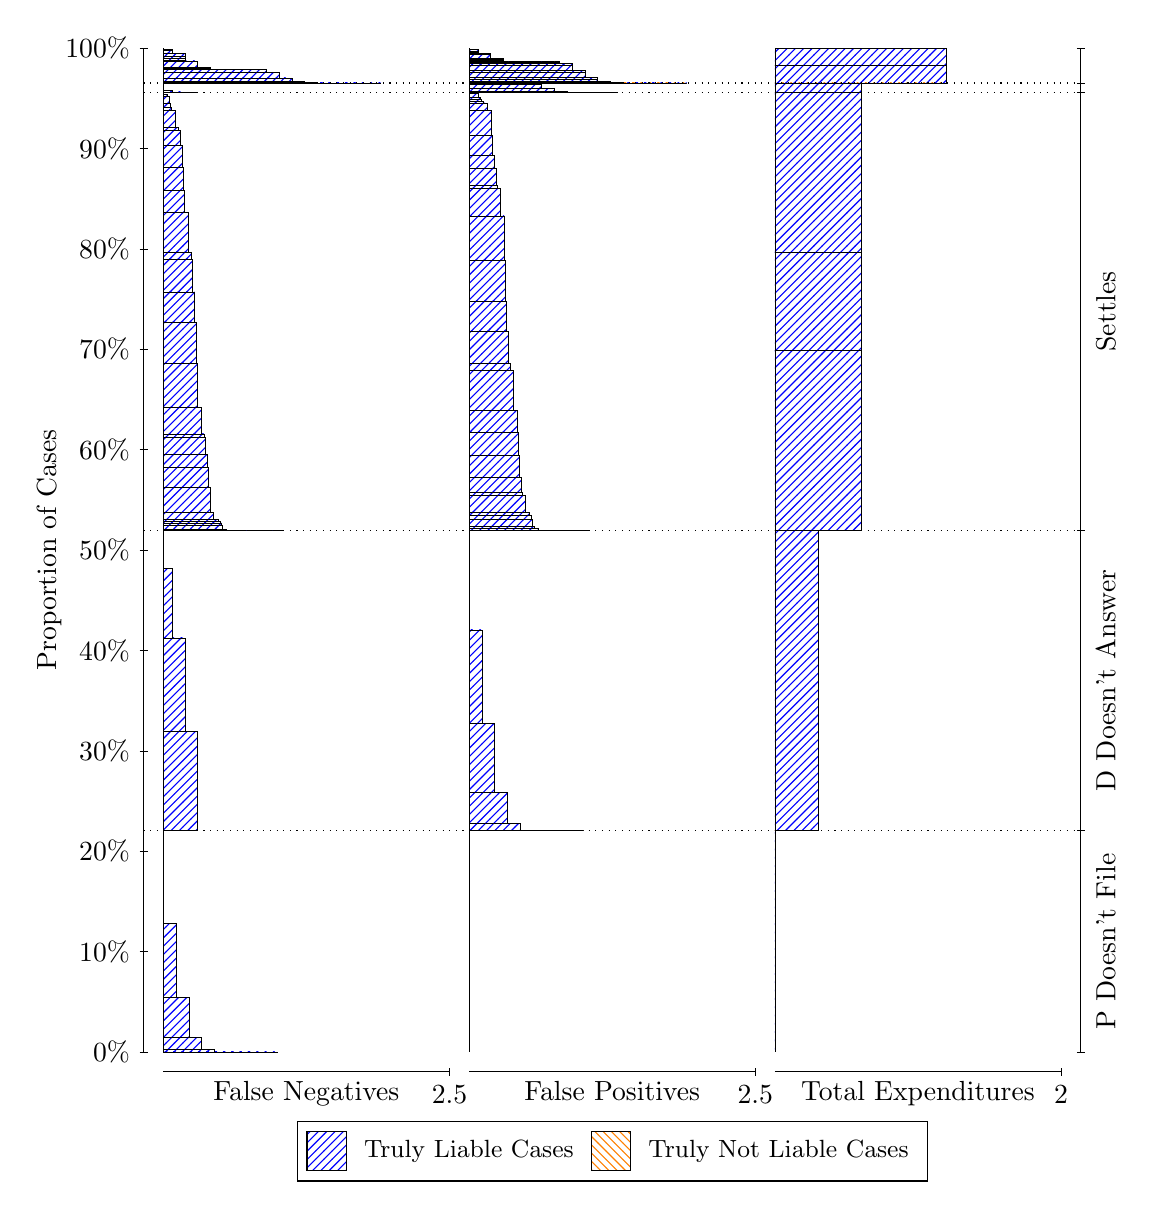
\begin{tikzpicture}
\draw[black, very thin] (1.5,1.75) -- (1.5,14.5);
\node[rotate=90, text=black, anchor=center] at (0.3, 8.125) {Proportion of Cases};
\draw[black, very thin] (1.45,1.75) -- (1.55,1.75);
\node[text=black, anchor=east] at (1.45, 1.75) {0\%};
\draw[black, very thin] (1.45,3.025) -- (1.55,3.025);
\node[text=black, anchor=east] at (1.45, 3.025) {10\%};
\draw[black, very thin] (1.45,4.3) -- (1.55,4.3);
\node[text=black, anchor=east] at (1.45, 4.3) {20\%};
\draw[black, very thin] (1.45,5.575) -- (1.55,5.575);
\node[text=black, anchor=east] at (1.45, 5.575) {30\%};
\draw[black, very thin] (1.45,6.85) -- (1.55,6.85);
\node[text=black, anchor=east] at (1.45, 6.85) {40\%};
\draw[black, very thin] (1.45,8.125) -- (1.55,8.125);
\node[text=black, anchor=east] at (1.45, 8.125) {50\%};
\draw[black, very thin] (1.45,9.4) -- (1.55,9.4);
\node[text=black, anchor=east] at (1.45, 9.4) {60\%};
\draw[black, very thin] (1.45,10.675) -- (1.55,10.675);
\node[text=black, anchor=east] at (1.45, 10.675) {70\%};
\draw[black, very thin] (1.45,11.95) -- (1.55,11.95);
\node[text=black, anchor=east] at (1.45, 11.95) {80\%};
\draw[black, very thin] (1.45,13.225) -- (1.55,13.225);
\node[text=black, anchor=east] at (1.45, 13.225) {90\%};
\draw[black, very thin] (1.45,14.5) -- (1.55,14.5);
\node[text=black, anchor=east] at (1.45, 14.5) {100\%};

\draw[black, very thin] (13.4,1.75) -- (13.4,14.5);
\draw[black, very thin] (13.35,1.75) -- (13.45,1.75);
\node[anchor=west] at (13.35, 1.75) {};
\draw[black, very thin] (13.35,4.5603) -- (13.45,4.5603);
\node[anchor=west] at (13.35, 4.5603) {};
\draw[black, very thin] (13.35,8.3729) -- (13.45,8.3729);
\node[anchor=west] at (13.35, 8.3729) {};
\draw[black, very thin] (13.35,13.94) -- (13.45,13.94);
\node[anchor=west] at (13.35, 13.94) {};
\draw[black, very thin] (13.35,14.056) -- (13.45,14.056);
\node[anchor=west] at (13.35, 14.056) {};
\draw[black, very thin] (13.35,14.5) -- (13.45,14.5);
\node[anchor=west] at (13.35, 14.5) {};

\draw[black, very thin, pattern color=blue, pattern=north east lines] (1.75,1.75) rectangle (3.2033,1.75);
\draw[black, very thin, pattern color=blue, pattern=north east lines] (1.75,1.75) rectangle (3.0419,1.75);
\draw[black, very thin, pattern color=blue, pattern=north east lines] (1.75,1.75) rectangle (2.8804,1.75);
\draw[black, very thin, pattern color=blue, pattern=north east lines] (1.75,1.75) rectangle (2.7189,1.7501);
\draw[black, very thin, pattern color=blue, pattern=north east lines] (1.75,1.7501) rectangle (2.5574,1.7523);
\draw[black, very thin, pattern color=blue, pattern=north east lines] (1.75,1.7523) rectangle (2.3959,1.779);
\draw[black, very thin, pattern color=blue, pattern=north east lines] (1.75,1.779) rectangle (2.2344,1.9392);
\draw[black, very thin, pattern color=blue, pattern=north east lines] (1.75,1.9392) rectangle (2.073,2.4471);
\draw[black, very thin, pattern color=blue, pattern=north east lines] (1.75,2.4471) rectangle (1.9115,3.3812);
\draw[black, very thin, pattern color=orange, pattern=north west lines] (1.75,3.3812) rectangle (1.75,3.3812);
\draw[black, very thin, pattern color=blue, pattern=north east lines] (1.75,3.3812) rectangle (1.75,4.5603);
\draw[black, very thin, pattern color=blue, pattern=north east lines] (1.75,4.5603) rectangle (2.186,5.8238);
\draw[black, very thin, pattern color=blue, pattern=north east lines] (1.75,5.8238) rectangle (2.0245,7.0076);
\draw[black, very thin, pattern color=blue, pattern=north east lines] (1.75,7.0076) rectangle (1.863,7.8867);
\draw[black, very thin, pattern color=orange, pattern=north west lines] (1.75,7.8867) rectangle (1.75,7.8867);
\draw[black, very thin, pattern color=blue, pattern=north east lines] (1.75,7.8867) rectangle (1.75,8.3729);
\draw[black, very thin, pattern color=blue, pattern=north east lines] (1.75,8.3729) rectangle (3.276,8.3729);
\draw[black, very thin, pattern color=blue, pattern=north east lines] (1.75,8.3729) rectangle (3.1307,8.3729);
\draw[black, very thin, pattern color=blue, pattern=north east lines] (1.75,8.3729) rectangle (3.1145,8.3729);
\draw[black, very thin, pattern color=blue, pattern=north east lines] (1.75,8.3729) rectangle (2.9853,8.3729);
\draw[black, very thin, pattern color=blue, pattern=north east lines] (1.75,8.3729) rectangle (2.9692,8.3729);
\draw[black, very thin, pattern color=blue, pattern=north east lines] (1.75,8.3729) rectangle (2.953,8.3729);
\draw[black, very thin, pattern color=blue, pattern=north east lines] (1.75,8.3729) rectangle (2.9127,8.3729);
\draw[black, very thin, pattern color=blue, pattern=north east lines] (1.75,8.3729) rectangle (2.8239,8.373);
\draw[black, very thin, pattern color=blue, pattern=north east lines] (1.75,8.373) rectangle (2.8077,8.373);
\draw[black, very thin, pattern color=blue, pattern=north east lines] (1.75,8.373) rectangle (2.7916,8.373);
\draw[black, very thin, pattern color=blue, pattern=north east lines] (1.75,8.373) rectangle (2.7673,8.373);
\draw[black, very thin, pattern color=blue, pattern=north east lines] (1.75,8.373) rectangle (2.7512,8.373);
\draw[black, very thin, pattern color=blue, pattern=north east lines] (1.75,8.373) rectangle (2.6624,8.3748);
\draw[black, very thin, pattern color=blue, pattern=north east lines] (1.75,8.3748) rectangle (2.6462,8.3758);
\draw[black, very thin, pattern color=blue, pattern=north east lines] (1.75,8.3758) rectangle (2.6301,8.3761);
\draw[black, very thin, pattern color=blue, pattern=north east lines] (1.75,8.3761) rectangle (2.6059,8.3767);
\draw[black, very thin, pattern color=blue, pattern=north east lines] (1.75,8.3767) rectangle (2.5897,8.3768);
\draw[black, very thin, pattern color=blue, pattern=north east lines] (1.75,8.3768) rectangle (2.5493,8.3881);
\draw[black, very thin, pattern color=blue, pattern=north east lines] (1.75,8.3881) rectangle (2.5009,8.4364);
\draw[black, very thin, pattern color=blue, pattern=north east lines] (1.75,8.4364) rectangle (2.4847,8.4695);
\draw[black, very thin, pattern color=blue, pattern=north east lines] (1.75,8.4695) rectangle (2.4686,8.4865);
\draw[black, very thin, pattern color=blue, pattern=north east lines] (1.75,8.4865) rectangle (2.4444,8.5108);
\draw[black, very thin, pattern color=blue, pattern=north east lines] (1.75,8.5108) rectangle (2.4282,8.5153);
\draw[black, very thin, pattern color=blue, pattern=north east lines] (1.75,8.5153) rectangle (2.3879,8.6036);
\draw[black, very thin, pattern color=blue, pattern=north east lines] (1.75,8.6036) rectangle (2.3394,8.9188);
\draw[black, very thin, pattern color=blue, pattern=north east lines] (1.75,8.9188) rectangle (2.3233,9.1773);
\draw[black, very thin, pattern color=blue, pattern=north east lines] (1.75,9.1773) rectangle (2.3071,9.3405);
\draw[black, very thin, pattern color=blue, pattern=north east lines] (1.75,9.3405) rectangle (2.2829,9.5557);
\draw[black, very thin, pattern color=blue, pattern=north east lines] (1.75,9.5557) rectangle (2.2667,9.5997);
\draw[black, very thin, pattern color=blue, pattern=north east lines] (1.75,9.5997) rectangle (2.2264,9.9438);
\draw[black, very thin, pattern color=blue, pattern=north east lines] (1.75,9.9438) rectangle (2.1779,10.502);
\draw[black, very thin, pattern color=blue, pattern=north east lines] (1.75,10.502) rectangle (2.1618,11.023);
\draw[black, very thin, pattern color=blue, pattern=north east lines] (1.75,11.023) rectangle (2.1456,11.404);
\draw[black, very thin, pattern color=blue, pattern=north east lines] (1.75,11.404) rectangle (2.1214,11.822);
\draw[black, very thin, pattern color=blue, pattern=north east lines] (1.75,11.822) rectangle (2.1053,11.911);
\draw[black, very thin, pattern color=blue, pattern=north east lines] (1.75,11.911) rectangle (2.0649,12.411);
\draw[black, very thin, pattern color=blue, pattern=north east lines] (1.75,12.411) rectangle (2.0164,12.689);
\draw[black, very thin, pattern color=blue, pattern=north east lines] (1.75,12.689) rectangle (2.0003,12.986);
\draw[black, very thin, pattern color=blue, pattern=north east lines] (1.75,12.986) rectangle (1.9841,13.265);
\draw[black, very thin, pattern color=blue, pattern=north east lines] (1.75,13.265) rectangle (1.9599,13.457);
\draw[black, very thin, pattern color=blue, pattern=north east lines] (1.75,13.457) rectangle (1.9438,13.495);
\draw[black, very thin, pattern color=blue, pattern=north east lines] (1.75,13.495) rectangle (1.9034,13.707);
\draw[black, very thin, pattern color=blue, pattern=north east lines] (1.75,13.707) rectangle (1.855,13.744);
\draw[black, very thin, pattern color=blue, pattern=north east lines] (1.75,13.744) rectangle (1.8388,13.797);
\draw[black, very thin, pattern color=blue, pattern=north east lines] (1.75,13.797) rectangle (1.8227,13.889);
\draw[black, very thin, pattern color=blue, pattern=north east lines] (1.75,13.889) rectangle (1.7984,13.909);
\draw[black, very thin, pattern color=blue, pattern=north east lines] (1.75,13.909) rectangle (1.7823,13.912);
\draw[black, very thin, pattern color=orange, pattern=north west lines] (1.75,13.912) rectangle (1.75,13.912);
\draw[black, very thin, pattern color=blue, pattern=north east lines] (1.75,13.912) rectangle (1.75,13.94);
\draw[black, very thin, pattern color=blue, pattern=north east lines] (1.75,13.94) rectangle (2.186,13.94);
\draw[black, very thin, pattern color=blue, pattern=north east lines] (1.75,13.94) rectangle (2.0245,13.942);
\draw[black, very thin, pattern color=blue, pattern=north east lines] (1.75,13.942) rectangle (1.863,13.96);
\draw[black, very thin, pattern color=orange, pattern=north west lines] (1.75,13.96) rectangle (1.75,13.96);
\draw[black, very thin, pattern color=blue, pattern=north east lines] (1.75,13.96) rectangle (1.75,14.056);
\draw[black, very thin, pattern color=blue, pattern=north east lines] (1.75,14.056) rectangle (4.5113,14.056);
\draw[black, very thin, pattern color=blue, pattern=north east lines] (1.75,14.056) rectangle (4.3499,14.056);
\draw[black, very thin, pattern color=blue, pattern=north east lines] (1.75,14.056) rectangle (4.1884,14.056);
\draw[black, very thin, pattern color=blue, pattern=north east lines] (1.75,14.056) rectangle (4.0269,14.056);
\draw[black, very thin, pattern color=blue, pattern=north east lines] (1.75,14.056) rectangle (4.0269,14.056);
\draw[black, very thin, pattern color=blue, pattern=north east lines] (1.75,14.056) rectangle (3.8654,14.057);
\draw[black, very thin, pattern color=blue, pattern=north east lines] (1.75,14.057) rectangle (3.8654,14.057);
\draw[black, very thin, pattern color=blue, pattern=north east lines] (1.75,14.057) rectangle (3.7039,14.057);
\draw[black, very thin, pattern color=blue, pattern=north east lines] (1.75,14.057) rectangle (3.7039,14.059);
\draw[black, very thin, pattern color=blue, pattern=north east lines] (1.75,14.059) rectangle (3.5424,14.067);
\draw[black, very thin, pattern color=blue, pattern=north east lines] (1.75,14.067) rectangle (3.5424,14.074);
\draw[black, very thin, pattern color=blue, pattern=north east lines] (1.75,14.074) rectangle (3.381,14.111);
\draw[black, very thin, pattern color=blue, pattern=north east lines] (1.75,14.111) rectangle (3.381,14.121);
\draw[black, very thin, pattern color=blue, pattern=north east lines] (1.75,14.121) rectangle (3.2195,14.192);
\draw[black, very thin, pattern color=blue, pattern=north east lines] (1.75,14.192) rectangle (3.1549,14.192);
\draw[black, very thin, pattern color=blue, pattern=north east lines] (1.75,14.192) rectangle (3.058,14.224);
\draw[black, very thin, pattern color=blue, pattern=north east lines] (1.75,14.224) rectangle (2.9934,14.224);
\draw[black, very thin, pattern color=blue, pattern=north east lines] (1.75,14.224) rectangle (2.9934,14.224);
\draw[black, very thin, pattern color=blue, pattern=north east lines] (1.75,14.224) rectangle (2.8965,14.224);
\draw[black, very thin, pattern color=blue, pattern=north east lines] (1.75,14.224) rectangle (2.8965,14.228);
\draw[black, very thin, pattern color=blue, pattern=north east lines] (1.75,14.228) rectangle (2.8319,14.228);
\draw[black, very thin, pattern color=blue, pattern=north east lines] (1.75,14.228) rectangle (2.735,14.228);
\draw[black, very thin, pattern color=blue, pattern=north east lines] (1.75,14.228) rectangle (2.735,14.228);
\draw[black, very thin, pattern color=blue, pattern=north east lines] (1.75,14.228) rectangle (2.6704,14.228);
\draw[black, very thin, pattern color=blue, pattern=north east lines] (1.75,14.228) rectangle (2.5736,14.228);
\draw[black, very thin, pattern color=blue, pattern=north east lines] (1.75,14.228) rectangle (2.509,14.228);
\draw[black, very thin, pattern color=blue, pattern=north east lines] (1.75,14.228) rectangle (2.509,14.229);
\draw[black, very thin, pattern color=blue, pattern=north east lines] (1.75,14.229) rectangle (2.4121,14.229);
\draw[black, very thin, pattern color=blue, pattern=north east lines] (1.75,14.229) rectangle (2.3475,14.229);
\draw[black, very thin, pattern color=blue, pattern=north east lines] (1.75,14.229) rectangle (2.3475,14.232);
\draw[black, very thin, pattern color=blue, pattern=north east lines] (1.75,14.232) rectangle (2.3475,14.241);
\draw[black, very thin, pattern color=blue, pattern=north east lines] (1.75,14.241) rectangle (2.3475,14.253);
\draw[black, very thin, pattern color=blue, pattern=north east lines] (1.75,14.253) rectangle (2.186,14.253);
\draw[black, very thin, pattern color=blue, pattern=north east lines] (1.75,14.253) rectangle (2.186,14.338);
\draw[black, very thin, pattern color=blue, pattern=north east lines] (1.75,14.338) rectangle (2.0245,14.34);
\draw[black, very thin, pattern color=blue, pattern=north east lines] (1.75,14.34) rectangle (2.0245,14.367);
\draw[black, very thin, pattern color=blue, pattern=north east lines] (1.75,14.367) rectangle (2.0245,14.396);
\draw[black, very thin, pattern color=blue, pattern=north east lines] (1.75,14.396) rectangle (2.0245,14.43);
\draw[black, very thin, pattern color=blue, pattern=north east lines] (1.75,14.43) rectangle (1.863,14.437);
\draw[black, very thin, pattern color=blue, pattern=north east lines] (1.75,14.437) rectangle (1.863,14.469);
\draw[black, very thin, pattern color=blue, pattern=north east lines] (1.75,14.469) rectangle (1.863,14.48);
\draw[black, very thin, pattern color=orange, pattern=north west lines] (1.75,14.48) rectangle (1.75,14.48);
\draw[black, very thin, pattern color=blue, pattern=north east lines] (1.75,14.48) rectangle (1.75,14.5);
\draw[black, very thin, pattern color=orange, pattern=north west lines] (5.6333,1.75) rectangle (5.6333,1.75);
\draw[black, very thin, pattern color=blue, pattern=north east lines] (5.6333,1.75) rectangle (5.6333,4.5603);
\draw[black, very thin, pattern color=orange, pattern=north west lines] (5.6333,4.5603) rectangle (7.0867,4.5603);
\draw[black, very thin, pattern color=blue, pattern=north east lines] (5.6333,4.5603) rectangle (7.0867,4.5603);
\draw[black, very thin, pattern color=blue, pattern=north east lines] (5.6333,4.5603) rectangle (6.9252,4.5603);
\draw[black, very thin, pattern color=blue, pattern=north east lines] (5.6333,4.5603) rectangle (6.7637,4.5603);
\draw[black, very thin, pattern color=blue, pattern=north east lines] (5.6333,4.5603) rectangle (6.6022,4.5605);
\draw[black, very thin, pattern color=blue, pattern=north east lines] (5.6333,4.5605) rectangle (6.4407,4.5683);
\draw[black, very thin, pattern color=blue, pattern=north east lines] (5.6333,4.5683) rectangle (6.2793,4.6533);
\draw[black, very thin, pattern color=blue, pattern=north east lines] (5.6333,4.6533) rectangle (6.1178,5.0465);
\draw[black, very thin, pattern color=blue, pattern=north east lines] (5.6333,5.0465) rectangle (5.9563,5.9256);
\draw[black, very thin, pattern color=blue, pattern=north east lines] (5.6333,5.9256) rectangle (5.7948,7.1094);
\draw[black, very thin, pattern color=blue, pattern=north east lines] (5.6333,7.1094) rectangle (5.6333,8.3729);
\draw[black, very thin, pattern color=orange, pattern=north west lines] (5.6333,8.3729) rectangle (7.1593,8.3729);
\draw[black, very thin, pattern color=blue, pattern=north east lines] (5.6333,8.3729) rectangle (7.1593,8.3729);
\draw[black, very thin, pattern color=blue, pattern=north east lines] (5.6333,8.3729) rectangle (6.9979,8.3729);
\draw[black, very thin, pattern color=orange, pattern=north west lines] (5.6333,8.3729) rectangle (6.9413,8.3729);
\draw[black, very thin, pattern color=blue, pattern=north east lines] (5.6333,8.3729) rectangle (6.9413,8.3729);
\draw[black, very thin, pattern color=blue, pattern=north east lines] (5.6333,8.3729) rectangle (6.8364,8.3729);
\draw[black, very thin, pattern color=orange, pattern=north west lines] (5.6333,8.3729) rectangle (6.796,8.3729);
\draw[black, very thin, pattern color=blue, pattern=north east lines] (5.6333,8.3729) rectangle (6.796,8.3729);
\draw[black, very thin, pattern color=blue, pattern=north east lines] (5.6333,8.3729) rectangle (6.7799,8.373);
\draw[black, very thin, pattern color=orange, pattern=north west lines] (5.6333,8.373) rectangle (6.7233,8.373);
\draw[black, very thin, pattern color=blue, pattern=north east lines] (5.6333,8.373) rectangle (6.7233,8.373);
\draw[black, very thin, pattern color=blue, pattern=north east lines] (5.6333,8.373) rectangle (6.6749,8.3734);
\draw[black, very thin, pattern color=blue, pattern=north east lines] (5.6333,8.3734) rectangle (6.6345,8.3735);
\draw[black, very thin, pattern color=blue, pattern=north east lines] (5.6333,8.3735) rectangle (6.6184,8.3739);
\draw[black, very thin, pattern color=orange, pattern=north west lines] (5.6333,8.3739) rectangle (6.578,8.3739);
\draw[black, very thin, pattern color=blue, pattern=north east lines] (5.6333,8.3739) rectangle (6.578,8.3776);
\draw[black, very thin, pattern color=blue, pattern=north east lines] (5.6333,8.3776) rectangle (6.5619,8.379);
\draw[black, very thin, pattern color=blue, pattern=north east lines] (5.6333,8.379) rectangle (6.5134,8.4007);
\draw[black, very thin, pattern color=blue, pattern=north east lines] (5.6333,8.4007) rectangle (6.473,8.4039);
\draw[black, very thin, pattern color=blue, pattern=north east lines] (5.6333,8.4039) rectangle (6.4569,8.4238);
\draw[black, very thin, pattern color=orange, pattern=north west lines] (5.6333,8.4238) rectangle (6.4327,8.4238);
\draw[black, very thin, pattern color=blue, pattern=north east lines] (5.6333,8.4238) rectangle (6.4327,8.5155);
\draw[black, very thin, pattern color=blue, pattern=north east lines] (5.6333,8.5155) rectangle (6.4165,8.5685);
\draw[black, very thin, pattern color=blue, pattern=north east lines] (5.6333,8.5685) rectangle (6.4004,8.6057);
\draw[black, very thin, pattern color=blue, pattern=north east lines] (5.6333,8.6057) rectangle (6.3519,8.8179);
\draw[black, very thin, pattern color=blue, pattern=north east lines] (5.6333,8.8179) rectangle (6.3116,8.8551);
\draw[black, very thin, pattern color=blue, pattern=north east lines] (5.6333,8.8551) rectangle (6.2954,9.047);
\draw[black, very thin, pattern color=blue, pattern=north east lines] (5.6333,9.047) rectangle (6.2712,9.3264);
\draw[black, very thin, pattern color=blue, pattern=north east lines] (5.6333,9.3264) rectangle (6.255,9.6239);
\draw[black, very thin, pattern color=blue, pattern=north east lines] (5.6333,9.6239) rectangle (6.2389,9.9014);
\draw[black, very thin, pattern color=blue, pattern=north east lines] (5.6333,9.9014) rectangle (6.1904,10.402);
\draw[black, very thin, pattern color=blue, pattern=north east lines] (5.6333,10.402) rectangle (6.1501,10.491);
\draw[black, very thin, pattern color=blue, pattern=north east lines] (5.6333,10.491) rectangle (6.1339,10.909);
\draw[black, very thin, pattern color=blue, pattern=north east lines] (5.6333,10.909) rectangle (6.1097,11.289);
\draw[black, very thin, pattern color=blue, pattern=north east lines] (5.6333,11.289) rectangle (6.0936,11.81);
\draw[black, very thin, pattern color=blue, pattern=north east lines] (5.6333,11.81) rectangle (6.0774,12.369);
\draw[black, very thin, pattern color=blue, pattern=north east lines] (5.6333,12.369) rectangle (6.029,12.713);
\draw[black, very thin, pattern color=blue, pattern=north east lines] (5.6333,12.713) rectangle (5.9886,12.757);
\draw[black, very thin, pattern color=blue, pattern=north east lines] (5.6333,12.757) rectangle (5.9724,12.972);
\draw[black, very thin, pattern color=blue, pattern=north east lines] (5.6333,12.972) rectangle (5.9482,13.135);
\draw[black, very thin, pattern color=blue, pattern=north east lines] (5.6333,13.135) rectangle (5.9321,13.394);
\draw[black, very thin, pattern color=blue, pattern=north east lines] (5.6333,13.394) rectangle (5.9159,13.709);
\draw[black, very thin, pattern color=blue, pattern=north east lines] (5.6333,13.709) rectangle (5.8675,13.797);
\draw[black, very thin, pattern color=blue, pattern=north east lines] (5.6333,13.797) rectangle (5.8271,13.802);
\draw[black, very thin, pattern color=blue, pattern=north east lines] (5.6333,13.802) rectangle (5.811,13.826);
\draw[black, very thin, pattern color=blue, pattern=north east lines] (5.6333,13.826) rectangle (5.7867,13.843);
\draw[black, very thin, pattern color=blue, pattern=north east lines] (5.6333,13.843) rectangle (5.7706,13.876);
\draw[black, very thin, pattern color=blue, pattern=north east lines] (5.6333,13.876) rectangle (5.7544,13.924);
\draw[black, very thin, pattern color=blue, pattern=north east lines] (5.6333,13.924) rectangle (5.706,13.936);
\draw[black, very thin, pattern color=blue, pattern=north east lines] (5.6333,13.936) rectangle (5.6656,13.936);
\draw[black, very thin, pattern color=blue, pattern=north east lines] (5.6333,13.936) rectangle (5.6495,13.936);
\draw[black, very thin, pattern color=blue, pattern=north east lines] (5.6333,13.936) rectangle (5.6333,13.94);
\draw[black, very thin, pattern color=orange, pattern=north west lines] (5.6333,13.94) rectangle (7.5227,13.94);
\draw[black, very thin, pattern color=blue, pattern=north east lines] (5.6333,13.94) rectangle (7.5227,13.94);
\draw[black, very thin, pattern color=blue, pattern=north east lines] (5.6333,13.94) rectangle (7.3612,13.94);
\draw[black, very thin, pattern color=blue, pattern=north east lines] (5.6333,13.94) rectangle (7.1997,13.94);
\draw[black, very thin, pattern color=blue, pattern=north east lines] (5.6333,13.94) rectangle (7.0382,13.94);
\draw[black, very thin, pattern color=blue, pattern=north east lines] (5.6333,13.94) rectangle (6.8767,13.945);
\draw[black, very thin, pattern color=blue, pattern=north east lines] (5.6333,13.945) rectangle (6.7153,13.983);
\draw[black, very thin, pattern color=blue, pattern=north east lines] (5.6333,13.983) rectangle (6.5538,14.036);
\draw[black, very thin, pattern color=blue, pattern=north east lines] (5.6333,14.036) rectangle (6.3923,14.054);
\draw[black, very thin, pattern color=blue, pattern=north east lines] (5.6333,14.054) rectangle (6.2308,14.056);
\draw[black, very thin, pattern color=blue, pattern=north east lines] (5.6333,14.056) rectangle (6.0693,14.056);
\draw[black, very thin, pattern color=orange, pattern=north west lines] (5.6333,14.056) rectangle (8.3947,14.056);
\draw[black, very thin, pattern color=blue, pattern=north east lines] (5.6333,14.056) rectangle (8.3947,14.056);
\draw[black, very thin, pattern color=orange, pattern=north west lines] (5.6333,14.056) rectangle (8.2332,14.056);
\draw[black, very thin, pattern color=blue, pattern=north east lines] (5.6333,14.056) rectangle (8.2332,14.056);
\draw[black, very thin, pattern color=orange, pattern=north west lines] (5.6333,14.056) rectangle (8.0717,14.056);
\draw[black, very thin, pattern color=blue, pattern=north east lines] (5.6333,14.056) rectangle (8.0717,14.056);
\draw[black, very thin, pattern color=blue, pattern=north east lines] (5.6333,14.056) rectangle (7.9102,14.056);
\draw[black, very thin, pattern color=orange, pattern=north west lines] (5.6333,14.056) rectangle (7.9102,14.056);
\draw[black, very thin, pattern color=blue, pattern=north east lines] (5.6333,14.056) rectangle (7.9102,14.056);
\draw[black, very thin, pattern color=orange, pattern=north west lines] (5.6333,14.056) rectangle (7.7487,14.056);
\draw[black, very thin, pattern color=blue, pattern=north east lines] (5.6333,14.056) rectangle (7.7487,14.057);
\draw[black, very thin, pattern color=blue, pattern=north east lines] (5.6333,14.057) rectangle (7.7487,14.057);
\draw[black, very thin, pattern color=orange, pattern=north west lines] (5.6333,14.057) rectangle (7.5873,14.057);
\draw[black, very thin, pattern color=blue, pattern=north east lines] (5.6333,14.057) rectangle (7.5873,14.06);
\draw[black, very thin, pattern color=blue, pattern=north east lines] (5.6333,14.06) rectangle (7.5873,14.06);
\draw[black, very thin, pattern color=blue, pattern=north east lines] (5.6333,14.06) rectangle (7.4258,14.064);
\draw[black, very thin, pattern color=orange, pattern=north west lines] (5.6333,14.064) rectangle (7.4258,14.064);
\draw[black, very thin, pattern color=blue, pattern=north east lines] (5.6333,14.064) rectangle (7.4258,14.077);
\draw[black, very thin, pattern color=blue, pattern=north east lines] (5.6333,14.077) rectangle (7.2643,14.101);
\draw[black, very thin, pattern color=blue, pattern=north east lines] (5.6333,14.101) rectangle (7.2643,14.126);
\draw[black, very thin, pattern color=blue, pattern=north east lines] (5.6333,14.126) rectangle (7.1028,14.191);
\draw[black, very thin, pattern color=blue, pattern=north east lines] (5.6333,14.191) rectangle (7.1028,14.218);
\draw[black, very thin, pattern color=blue, pattern=north east lines] (5.6333,14.218) rectangle (6.9413,14.285);
\draw[black, very thin, pattern color=blue, pattern=north east lines] (5.6333,14.285) rectangle (6.9413,14.303);
\draw[black, very thin, pattern color=blue, pattern=north east lines] (5.6333,14.303) rectangle (6.7799,14.316);
\draw[black, very thin, pattern color=blue, pattern=north east lines] (5.6333,14.316) rectangle (6.7799,14.325);
\draw[black, very thin, pattern color=blue, pattern=north east lines] (5.6333,14.325) rectangle (6.7799,14.327);
\draw[black, very thin, pattern color=orange, pattern=north west lines] (5.6333,14.327) rectangle (6.7153,14.327);
\draw[black, very thin, pattern color=blue, pattern=north east lines] (5.6333,14.327) rectangle (6.7153,14.327);
\draw[black, very thin, pattern color=blue, pattern=north east lines] (5.6333,14.327) rectangle (6.6184,14.328);
\draw[black, very thin, pattern color=blue, pattern=north east lines] (5.6333,14.328) rectangle (6.6184,14.329);
\draw[black, very thin, pattern color=orange, pattern=north west lines] (5.6333,14.329) rectangle (6.5538,14.329);
\draw[black, very thin, pattern color=blue, pattern=north east lines] (5.6333,14.329) rectangle (6.5538,14.329);
\draw[black, very thin, pattern color=blue, pattern=north east lines] (5.6333,14.329) rectangle (6.4569,14.329);
\draw[black, very thin, pattern color=blue, pattern=north east lines] (5.6333,14.329) rectangle (6.4569,14.329);
\draw[black, very thin, pattern color=blue, pattern=north east lines] (5.6333,14.329) rectangle (6.4569,14.329);
\draw[black, very thin, pattern color=blue, pattern=north east lines] (5.6333,14.329) rectangle (6.3923,14.329);
\draw[black, very thin, pattern color=orange, pattern=north west lines] (5.6333,14.329) rectangle (6.3923,14.329);
\draw[black, very thin, pattern color=blue, pattern=north east lines] (5.6333,14.329) rectangle (6.3923,14.329);
\draw[black, very thin, pattern color=blue, pattern=north east lines] (5.6333,14.329) rectangle (6.2954,14.329);
\draw[black, very thin, pattern color=blue, pattern=north east lines] (5.6333,14.329) rectangle (6.2954,14.329);
\draw[black, very thin, pattern color=blue, pattern=north east lines] (5.6333,14.329) rectangle (6.2308,14.33);
\draw[black, very thin, pattern color=orange, pattern=north west lines] (5.6333,14.33) rectangle (6.2308,14.33);
\draw[black, very thin, pattern color=blue, pattern=north east lines] (5.6333,14.33) rectangle (6.2308,14.33);
\draw[black, very thin, pattern color=blue, pattern=north east lines] (5.6333,14.33) rectangle (6.2308,14.332);
\draw[black, very thin, pattern color=blue, pattern=north east lines] (5.6333,14.332) rectangle (6.1339,14.332);
\draw[black, very thin, pattern color=blue, pattern=north east lines] (5.6333,14.332) rectangle (6.0693,14.347);
\draw[black, very thin, pattern color=orange, pattern=north west lines] (5.6333,14.347) rectangle (6.0693,14.347);
\draw[black, very thin, pattern color=blue, pattern=north east lines] (5.6333,14.347) rectangle (6.0693,14.351);
\draw[black, very thin, pattern color=blue, pattern=north east lines] (5.6333,14.351) rectangle (6.0693,14.364);
\draw[black, very thin, pattern color=blue, pattern=north east lines] (5.6333,14.364) rectangle (5.9724,14.364);
\draw[black, very thin, pattern color=blue, pattern=north east lines] (5.6333,14.364) rectangle (5.9079,14.415);
\draw[black, very thin, pattern color=blue, pattern=north east lines] (5.6333,14.415) rectangle (5.9079,14.435);
\draw[black, very thin, pattern color=blue, pattern=north east lines] (5.6333,14.435) rectangle (5.7464,14.442);
\draw[black, very thin, pattern color=blue, pattern=north east lines] (5.6333,14.442) rectangle (5.7464,14.458);
\draw[black, very thin, pattern color=blue, pattern=north east lines] (5.6333,14.458) rectangle (5.7464,14.482);
\draw[black, very thin, pattern color=blue, pattern=north east lines] (5.6333,14.482) rectangle (5.6333,14.5);
\draw[black, very thin, pattern color=orange, pattern=north west lines] (9.5167,1.75) rectangle (9.5167,1.75);
\draw[black, very thin, pattern color=blue, pattern=north east lines] (9.5167,1.75) rectangle (9.5167,4.5603);
\draw[black, very thin, pattern color=orange, pattern=north west lines] (9.5167,4.5603) rectangle (10.062,4.5603);
\draw[black, very thin, pattern color=blue, pattern=north east lines] (9.5167,4.5603) rectangle (10.062,8.3729);
\draw[black, very thin, pattern color=orange, pattern=north west lines] (9.5167,8.3729) rectangle (10.607,8.3729);
\draw[black, very thin, pattern color=blue, pattern=north east lines] (9.5167,8.3729) rectangle (10.607,10.662);
\draw[black, very thin, pattern color=orange, pattern=north west lines] (9.5167,10.662) rectangle (10.607,10.662);
\draw[black, very thin, pattern color=blue, pattern=north east lines] (9.5167,10.662) rectangle (10.607,11.902);
\draw[black, very thin, pattern color=orange, pattern=north west lines] (9.5167,11.902) rectangle (10.607,11.902);
\draw[black, very thin, pattern color=blue, pattern=north east lines] (9.5167,11.902) rectangle (10.607,13.94);
\draw[black, very thin, pattern color=orange, pattern=north west lines] (9.5167,13.94) rectangle (10.607,13.94);
\draw[black, very thin, pattern color=blue, pattern=north east lines] (9.5167,13.94) rectangle (10.607,14.056);
\draw[black, very thin, pattern color=orange, pattern=north west lines] (9.5167,14.056) rectangle (11.697,14.056);
\draw[black, very thin, pattern color=blue, pattern=north east lines] (9.5167,14.056) rectangle (11.697,14.283);
\draw[black, very thin, pattern color=orange, pattern=north west lines] (9.5167,14.283) rectangle (11.697,14.283);
\draw[black, very thin, pattern color=blue, pattern=north east lines] (9.5167,14.283) rectangle (11.697,14.5);
\draw[black, dotted] (1.5,4.5603) -- (13.4,4.5603);
\draw[black, dotted] (1.5,8.3729) -- (13.4,8.3729);
\draw[black, dotted] (1.5,13.94) -- (13.4,13.94);
\draw[black, dotted] (1.5,14.056) -- (13.4,14.056);
\draw[black, very thin] (1.75,1.5) -- (5.3833,1.5);
\node[text=black, anchor=north] at (3.5667, 1.5) {False Negatives};
\draw[black, very thin] (5.3833,1.45) -- (5.3833,1.55);
\node[text=black, anchor=north] at (5.3833, 1.45) {2.5};

\draw[black, very thin] (5.6333,1.5) -- (9.2667,1.5);
\node[text=black, anchor=north] at (7.45, 1.5) {False Positives};
\draw[black, very thin] (9.2667,1.45) -- (9.2667,1.55);
\node[text=black, anchor=north] at (9.2667, 1.45) {2.5};

\draw[black, very thin] (9.5167,1.5) -- (13.15,1.5);
\node[text=black, anchor=north] at (11.333, 1.5) {Total Expenditures};
\draw[black, very thin] (13.15,1.45) -- (13.15,1.55);
\node[text=black, anchor=north] at (13.15, 1.45) {2};

\node[text=black, centered, rotate=90] at (13.72, 3.1551) {P Doesn't File};
\node[text=black, centered, rotate=90] at (13.72, 6.4666) {D Doesn't Answer};
\node[text=black, centered, rotate=90] at (13.72, 11.156) {Settles};



\draw (7.449999999999999,1.5) node[draw=none] (baseCoordinate) {};
\begin{scope}[align=center]
        \matrix[scale=0.5, draw=black, below=0.5cm of baseCoordinate, nodes={draw}, column sep=0.1cm]{
            \node[rectangle, draw, minimum width=0.5cm, minimum height=0.5cm, pattern color=blue, pattern=north east lines] {}; &
            \node[draw=none, font=\small, text=black] (B) {Truly Liable Cases}; &
            \node[rectangle, draw, minimum width=0.5cm, minimum height=0.5cm, pattern color=orange, pattern=north west lines] {}; &
            \node[draw=none, font=\small, text=black] (B) {Truly Not Liable Cases}; \\
            };
\end{scope}

\end{tikzpicture}
\end{document}